\documentclass[10pt,border=3mm,tikz]{standalone}
\usetikzlibrary{arrows.meta}

\begin{document}
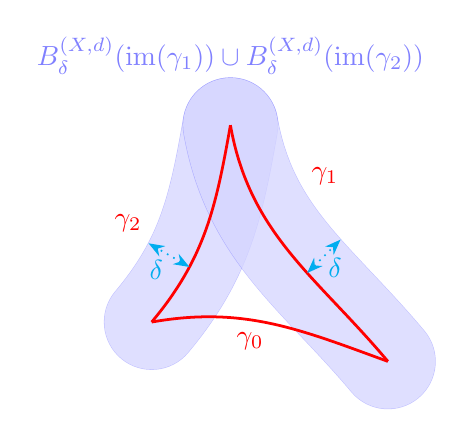
\begin{tikzpicture}[
    inner/.style={red,line width = 1pt,},
    outer/.style={double distance=12mm,
                  line cap=round,
                  blue!50,          % deal with overdrawings
                  opacity=.5,       % deal with overdrawings
                  line width=.2pt},
    > = {Stealth},                  % nicer arrow tip
    arr/.style={<->,cyan,dotted,line width=.6pt},
 ]
    % ~~~ the 3 points ~~~~~~~~~~~~~
    \coordinate (A) at (0,0);
    \coordinate (B) at (3,-.5);
    \coordinate (C) at (1,2.5);
    
    % ~~~ lines ~~~~~~~~~~~~~
    \draw[outer] (A) to[out= 50,in=260] (C);
    \draw[outer] (B) to[out=130,in=280] (C);
    \node[label={[text = blue!50]$B_\delta^{(X,d)}(\textup{im}(\gamma_1))\cup B_\delta^{(X,d)}(\textup{im}(\gamma_2))$}] at (1,2.9) {};

    % - - remember some points - - - - -
    \draw[inner] (A) to[out= 10,in=160] coordinate [pos=.55] (A1) (B);
    \node[label={[text = red]$\gamma_0$}] at (1.25,-0.6) {};
    \draw[inner] (A) to[out= 50,in=260] coordinate [pos=.30] (C1) (C);
    \node[label={[text = red]$\gamma_1$}] at (2.2,1.5) {};
    \draw[inner] (B) to[out=130,in=280] coordinate [pos=.40] (B1) (C);
    \node[label={[text = red]$\gamma_2$}] at (-0.3,0.9) {};
    
    % ~~~ the deltas ~~~~~~~~~~~~~~~
%   \node at (A1) {X};  % testing the positions
%   \node at (B1) {X};
%   \node at (C1) {X};
    \draw[arr] (B1) -- node[shift=(-45:.2)] {$\delta$} +( 45:.6);
    \draw[arr] (C1) -- node[shift=(230:.25)] {$\delta$} +(150:.6);
 \end{tikzpicture}
\end{document}